\section{Alpha 5}

Dans cette section, nous montrerons le résultat suivant, obtenu pendant mon stage avec Cyril Gavoille.

\begin{theorem}\label{alpha5borne}

$$\alpha_5 < 3.603564775$$

\end{theorem}

Dans la suite on appellera $P$ l'ensemble des points représentant les robots endormis et on considérera $\gamma$ la fonction qui à un ensemble de points associe le temps de réveil du problème associé. Pour cela, on prouvera le résultat suivant.

\begin{lemma}\label{chord}
Pour tout $P$ de taille 5, pour tout $\alpha \in \left]0, \frac{\pi}{2}\right[$, on a
$$\gamma(P) \leq \max\left(3 + \chord\left(\alpha\right), 1 + 2\chord\left(\frac{\pi}{2} - \frac{\alpha}{4}\right)\right)$$
où $\chord$ représente la longueur d'un arc de cercle de rayon 1 et d'angle $\theta$. On a donc $\chord(\theta) = 2\sin(\theta/2)$
\end{lemma}

\begin{proof}[Preuve de \ref{alpha5borne} en supposant Lemme \ref{chord}]

$\alpha \mapsto 3+\chord(\alpha)$ étant croissante $\alpha \mapsto 1 + 2\chord(\frac{\pi}{2} - \frac{\alpha}{4})$ étant décroissante, le minimum des deux fonctions est atteint en leur croisement qui se produit en une abscisse d'environ $0.6131233066$ et dont la valeur exacte n'est pas facilement calculable. Ainsi on a

\(\forall P, \gamma(P) < 3.603564775\)

Ce qui montre que $\alpha_5 < 3.603564775$

\end{proof}

\begin{lemma}\label{worstchord}
Pour tout $n$ et $x_1$, $x_2$, ..., $x_n$ des points sur un arc de demi-cercle dans l'ordre. Alors le chemin $x_1$ - $x_2$ - ... - $x_n$ est le plus long lorsque les points sont uniformément répartis sur l' arc de demi-cercle.
\end{lemma}
\begin{proof}
On commence par identifier les points par l'angle qui les sépare d'une des deux extrémités, obtenant ainsi une suite $\left(\theta_k\right)$ identifiant nos points. Dès lors, la longueur du chemin est:

$$2\sum_{k=1}^{n-1} \sin\left(\frac{\theta_{k+1} - \theta_k}{2}\right)$$

Or $\frac{\theta_{k+1} - \theta_k}{2} \in ]0, \frac{\pi}{2}[$

Nous sommes donc sur un intervalle où $\sin$ est concave. Ainsi égaliser les $\frac{\theta_{k+1} - \theta_k}{2}$ conduit à la somme maximale et donc la longueur maximale du chemin. 
Cela implique alors que la distance entre tous les points est la même et vu qu'il est toujours préférable d'avoir des points aux extremités, on a donc que le pire cas est d'avoir les points uniformément répartis sur l'arc de demi-cercle.

\end{proof}

Dans la suite, on utilisera la notation $\gamma(T, P)$ pour donner le temps de réveil de P suivant l'arbre de réveil T.
On a alors $\forall P, \gamma(P) = \min_T(\gamma(T,P))$
et donc $\forall P, \forall T, \gamma(P) \leq \gamma(T, P)$

\subsection{Description des Cas}

La preuve fonctionne en trouvant pour chaque cas un arbre dont la longueur est au pire plus petite ou égale à la borne souhaitée.

\begin{itemize}
	\item \ref{conv5} Enveloppe convexe de taille 5
	\begin{itemize}
		\item \ref{1cas} Deux points dans un cône d'angle $\alpha$
		en particulier, cela traite du cas où il existe 2 points dans $A$, $B$, $C$ ou $D$.
		\item \ref{2cas} $|D| = 0$
		\item \ref{3cas} $|B| = |C| = 0$ (et $|D| = |A| = 1$)
		sans perte de généralité, on suppose que le point de $D$ appartient au demi-cercle du haut
		\begin{itemize}
			\item \ref{3cas1} le deuxième point du haut est entre $A$ et $B$
			il reste à décider de la position des points du bas
			\begin{itemize}
				\item \ref{3cas11} 1 point du bas entre $A$ et $C$ ainsi que le dernier entre $C$ et $D$.
				\item \ref{3cas12} 2 points entre $C$ et $D$
				\item \ref{3cas13} 2 points entre $A$ et $C$
			\end{itemize}
			\item \ref{3cas2} le deuxième point du haut est entre $B$ et $D$
			de même il reste à décider de la position des points du bas
			\begin{itemize}
				\item \ref{3cas21} 2 points entre $A$ et $C$
				\item \ref{3cas22} 2 points entre $C$ et $D$
				\item \ref{3cas23} 1 point dans chacune des deux zones
			\end{itemize}
		\end{itemize}
		\item \ref{4cas} $|A| = |B| = |C| = |D| = 1$
		\begin{itemize}
			\item \ref{4cas1} si le 5 ème point est dans un cône diagonal d'angle $\alpha$
			\item \ref{4cas2} sinon
		\end{itemize}
		\item \ref{5cas} $|A| = |D| = 1$, $|C| = 0$ et $|D| = 1$
		par symétrie, le cas $|C| = 1$, $|D| = 0$ rentre aussi dans cette catégorie, concluant la disjonction présente
		\begin{itemize}
			\item \ref{5cas1} le point dans $D$ appartient au demi-cercle du haut
			\begin{itemize}
				\item \ref{5cas11} si on a en bas un point de chaque côté
				\item \ref{5cas12} si les deux point du bas sont entre $C$ et $D$
				\item \ref{5cas13} si les deux points du bas sont entre $A$ et $C$
			\end{itemize}
			\item \ref{5cas2} le point dans $D$ appartient au demi-cercle du bas
			on a donc 4 cas selon le positionnement du point en haut et en bas
			\begin{itemize}
				\item \ref{5cas21} Point du haut entre $A$ et $B$ et point du bas entre $A$ et $C$
				\item \ref{5cas22} Point du haut entre $A$ et $B$ et point du bas entre $C$ et $D$
				\item \ref{5cas23} Point du haut entre $B$ et $D$ et point du bas entre $C$ et $D$
				\item \ref{5cas24} Point du haut entre $B$ et $D$ et point du bas entre $A$ et $C$
			\end{itemize}
		\end{itemize}
	\end{itemize}
	\item \ref{conv3} Enveloppe convexe de taille 3 et 4
\end{itemize}

\subsection{Enveloppe convexe de taille 5}\label{conv5}

Soit $\alpha > 0$ et $P$ un ensemble de 5 points Tout d'abord on tournera notre figure en sélectionnant un point tel que son axe coupe le cercle en deux demi-cercles contenant chacun 2 points. Un tel point existe toujours.

\begin{figure}[h!]
  \centering
  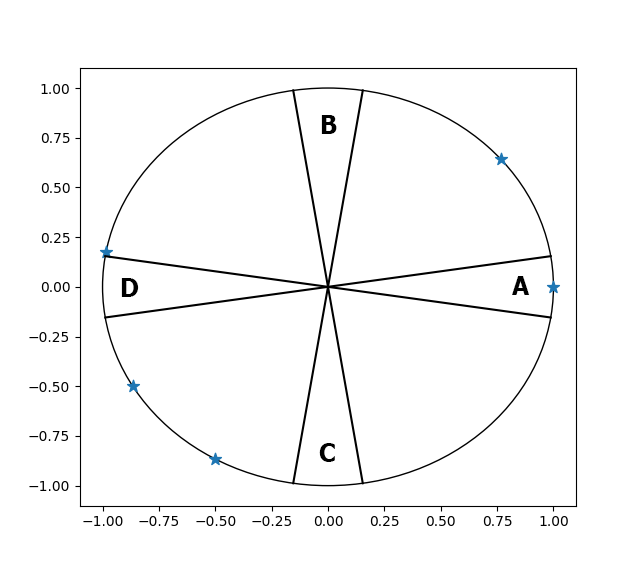
\includegraphics[scale=0.4]{initial_position}
  \caption{position initiale}
  \label{fig:initial_position}
\end{figure}

On sépare ensuite le cercle en différents cônes d'angle $\alpha$ nommés $A$,
$B$, $C$, et $D$ comme sur la figure \ref{fig:initial_position}. C'est en effet ce $\alpha$ qui apparaîtra dans la formule finale. On notera $|X|$ le nombre de point dans le cône $X$.

\subsubsection*{1er cas}\label{1cas} Supposons qu'il existe deux points inclus dans un cône d'angle $\alpha$

Dans ce cas, en réveillant les deux robots dans le cône avec celui initial, on peut aller réveiller les trois derniers où qu'ils soient dans le cercle. Réveiller les robots dans un cône d'angle $\alpha$ prend au plus un temps $1 + \chord(\alpha)$.
On peut donc réveiller tout le monde avec $\gamma(P) \leq 1 + \chord(\alpha) + 2 = 3 + \chord(\alpha)$

\subsubsection*{2ème cas}\label{2cas} $|D| = 0$

On prend $T$ l'arbre commençant au noeud de $A$ et explorant de part et d'autre de son axe en commençant par le noeud le plus proche.
Soit $P'$ l'ensemble de point sur le cercle où les deux points des demi cercles sont répartis entre $A$ et $D$.
On a $\gamma(P) \leq  \gamma(T, P) \leq \gamma(T, P')$

\begin{figure}[h!]
  \centering
  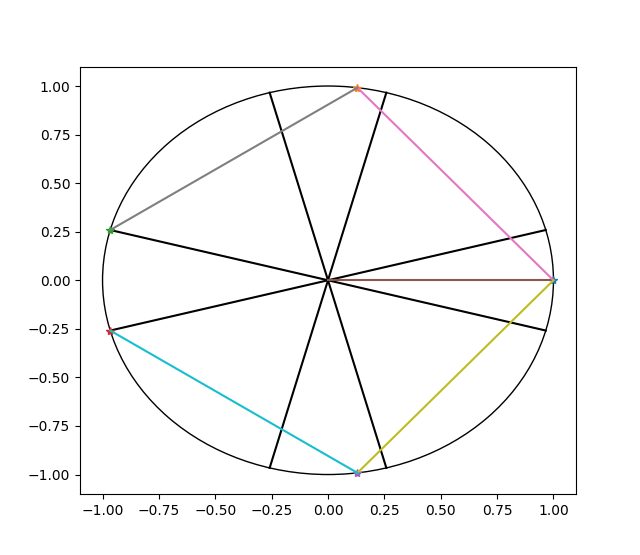
\includegraphics[scale=0.4]{2eme_cas}
  \caption{Résolution 2e cas}
  \label{fig:2eme_cas}
\end{figure}

En effet, d'après \ref{worstchord} le pire cas pour $P$ est d'avoir un point le plus loin possible de A et d'avoir des arcs égaux, positionnant donc le dernier point du demi-cercle pile entre le point de $A$ et celui collant $D$. On a alors

$\gamma(P) \leq \gamma(T, P') = 1 + 2\chord(\frac{\pi}{2} - \frac{\alpha}{4})$

\subsubsection*{3ème cas}\label{3cas} $|B| = |C| = 0$ ($|A| = 1$ et $|D| = 1$)
Par symétrie, on peut considérer que le point dans $D$ appartient au demi-cercle du haut et donc que l'on a un seul point en haut qui ne soit pas dans $D$ que l'on nommera $b$.

\begin{itemize}

\item \label{3cas1} Si $b$ est entre $A$ et $B$

\begin{itemize}

\item \label{3cas11} si $b$ entre $A$ et $B$ et il y a en bas 1 point de chaque côté

on choisit pour T l'arbre commençant en bas à gauche et séparant le travail des robots en 2 comme avant.
On prend ensuite le pire cas possible pour ce T.

\begin{figure}[h!]
  \centering
  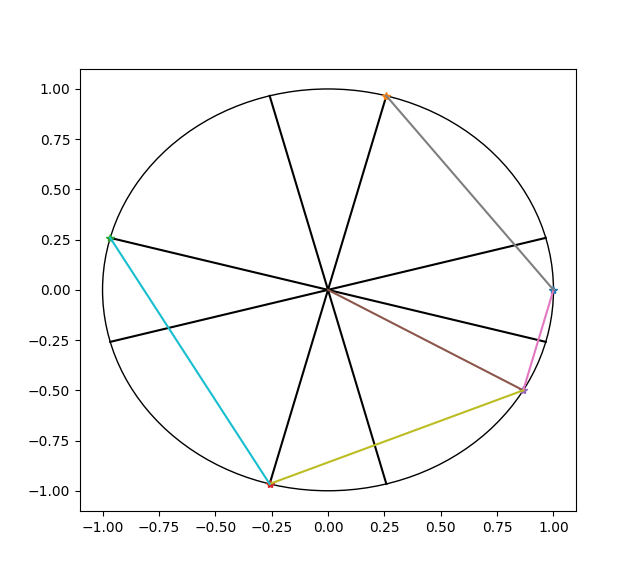
\includegraphics[scale=0.4]{3eme_cas1}
  \caption{Résolution 3e cas n1}
  \label{fig:3eme_cas1}
\end{figure}

En oubliant pas que l'angle entre $a$ et le point en bas à gauche est d'au moins $\alpha$ on peut donc appliquer le lemme \ref{worstchord} afin de conclure
$\gamma(P) \leq 1 + 2\chord(\frac{\pi}{2} - \frac{\alpha}{4})$

\item \label{3cas12} si $b$ entre $A$ et $B$ et deux points entre $C$ et $D$
l'arbre est le suivant:

\begin{figure}[h!]
  \centering
  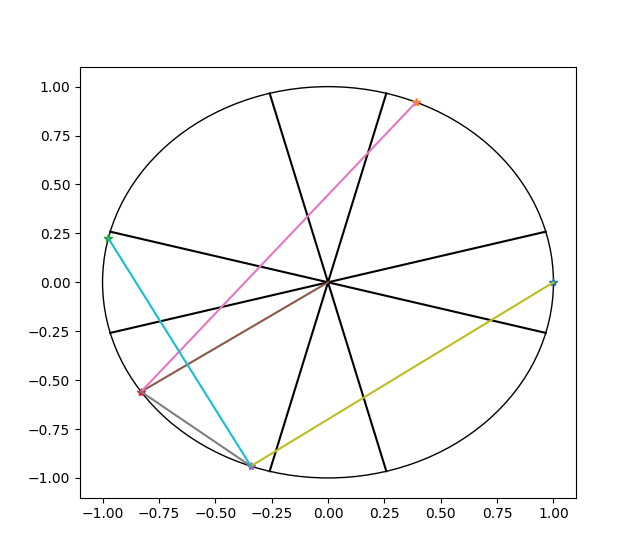
\includegraphics[scale=0.4]{3eme_cas2}
  \caption{Résolution 3e cas n2}
  \label{fig:3eme_cas2}
\end{figure}

Ici on néglige la branche rose car elle a une longueur totale de 3 (ce sera aussi fait dans les cas suivants)
La longueur de la branche bleue est ici $\leq 1+\chord\left(\frac{\pi}{2} - \alpha\right)+\chord(\frac{\pi}{2}) \leq 1 + 2\chord(\frac{\pi}{2} - \frac{\alpha}{4})$
Et pour la dernière branche, on applique \ref{worstchord} pour obtenir cette borne exacte

$=> \gamma(P) \leq 1 + 2\chord(\frac{\pi}{2} - \frac{\alpha}{4})$

\item \label{3cas13} Si $b$ entre $A$ et $B$ et deux points entre $A$ et $C$ on applique le même arbre

\end{itemize}

\item \label{3cas2} Si $b$ est entre $C$ et $D$

\begin{itemize}

\item \label{3cas21} Le seul cas difficile est celui où les deux points du bas sont entre $A$ et $C$.
suivant l'arbre suivant:

\begin{figure}[h!]
  \centering
  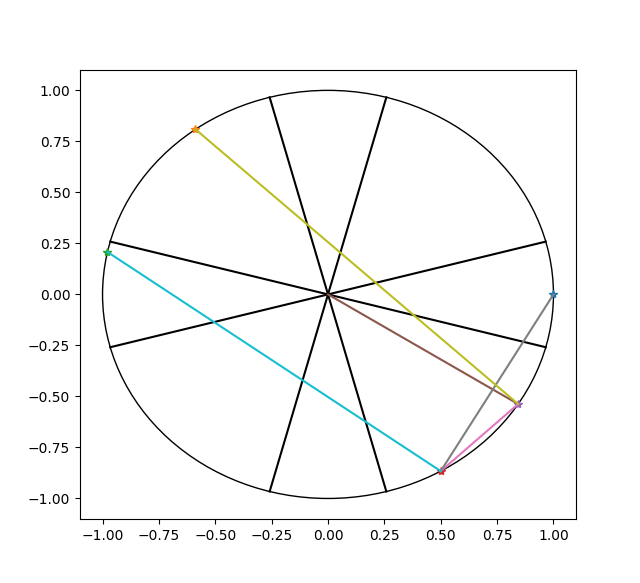
\includegraphics[scale=0.4]{3eme_cas3}
  \caption{Résolution 3e cas n3}
  \label{fig:3eme_cas3}
\end{figure}

La branche bleue ici se résout encore une fois par \ref{worstchord}
La branche jaune est négligée
et la branche violette permet le calcul de son pire cas en maximisant la longueur des cordes en respectant les contraintes angulaires. (en particulier que l'angle entre deux points doit être d'au moins $\alpha$)

on obtient alors
\begin{align*}
\gamma(P) &\leq \max\left(1+2\chord\left(\frac{\pi}{2} - \frac{\alpha}{4}\right), 1 + \chord\left(\frac{\pi}{2} - \frac{3\alpha}{2}\right) + \chord\left(\frac{\pi}{2} - \frac{\alpha}{2}\right)\right) \\
&\leq 1+2\chord\left(\frac{\pi}{2} - \frac{\alpha}{4}\right)
\end{align*}

\item \label{3cas22} Si l'on a 2 points entre $C$ et $D$, alors on peut effectuer l'arbre suivant

\begin{figure}[h!]
  \centering
  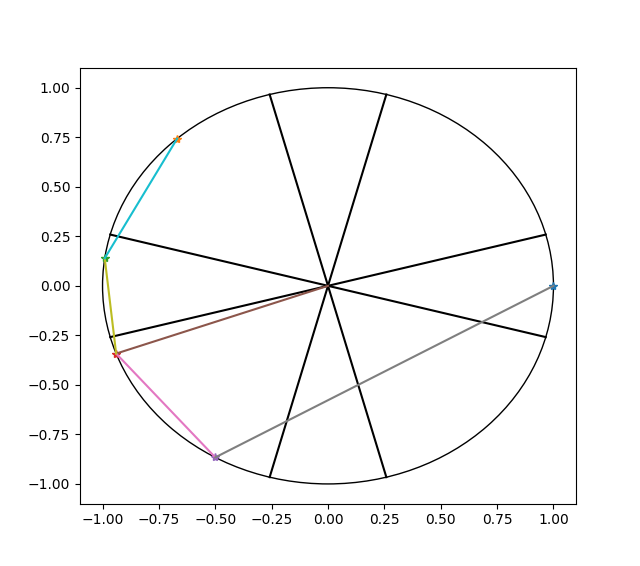
\includegraphics[scale=0.4]{3eme_cas4}
  \caption{Résolution 3e cas n4}
  \label{fig:3eme_cas4}
\end{figure}

On peut alors comme d'habitude utiliser \ref{worstchord} pour conclure

\item \label{3cas23} Pour dernier cas, nous avons 1 point de part et d'autre de la vertical en bas alors par un chemin similaire au point précédent:

\begin{figure}[h!]
  \centering
  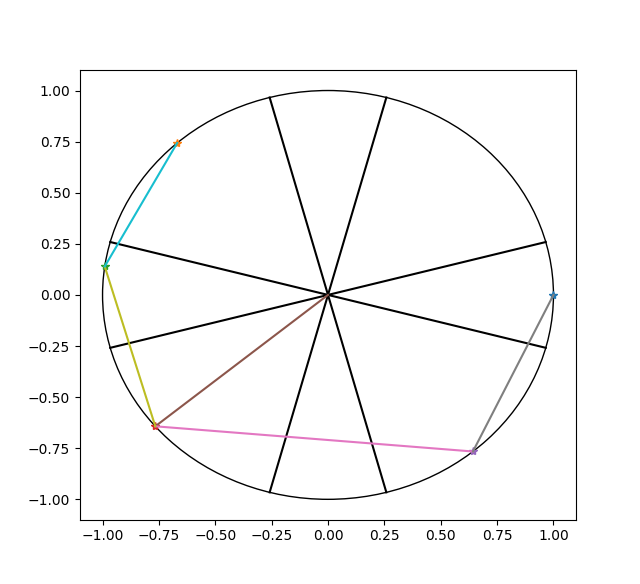
\includegraphics[scale=0.4]{3eme_cas5}
  \caption{Résolution 3e cas n5}
  \label{fig:3eme_cas5}
\end{figure}

Comme la dernière fois \ref{worstchord} nous permet de conclure

\end{itemize}
\end{itemize}

\subsubsection*{4eme cas}\label{4cas} $|A| = |B| = |C| = |D| = 1$

il reste donc un 5eme point à placer qui se trouve dans un des cônes diagonaux.

\begin{itemize}

\item \label{4cas1} si il est dans un cône d'angle $\alpha$ au centre du cône diagonal.

on a alors le chemin standard commençant par le 5ème point qui nous donne par \ref{worstchord}: $\gamma(P) \leq 1 + 2\chord(\frac{\pi}{2} - \frac{\alpha}{4})$

\item \label{4cas2} si ca n'est pas le cas alors on prend l'arbre commençant en ce 5 ème point mais allant vers le point le plus proche et le plus éloigné ainsi

\begin{figure}[h!]
  \centering
  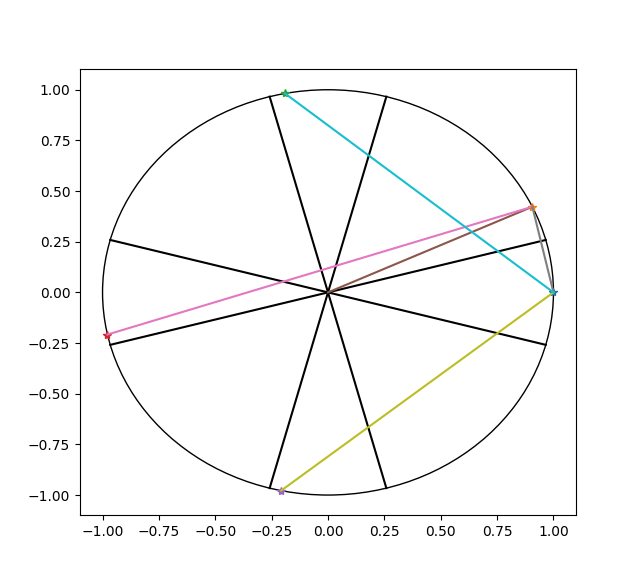
\includegraphics[scale=0.4]{4eme_cas}
  \caption{Résolution 4e cas}
  \label{fig:4eme_cas}
\end{figure}

La branche rose est négligée
la branche bleue est a sa première partie bornée par une corde de taille $\frac{\pi}{4}$ car le point du milieu est en dessous de la ligne diagonal d'un angle au moins $\frac{\alpha}{2}$ et la deuxième partie par $\frac{\pi}{2} + \alpha$
la branche jaune est symétrique à la branche bleue.

on a donc $\gamma(P) \leq 1 + \chord(\frac{\pi}{4}) + \chord(\frac{\pi}{2} + \alpha) \leq \max(3 + \chord(\alpha), 1 + 2\chord(\frac{\pi}{2} - \frac{\alpha}{4}))$

\end{itemize}

\subsubsection*{5ème cas}\label{5cas} $|B| = |A| = |D| = 1, |C| = 0$
à noter que par symétrie, ca s'applique pour $|B| = 0$ et $|C| = 1$

\begin{itemize}

\item \label{5cas1} Si le point dans D appartient au demi-cercle du haut:

\begin{itemize}

\item \label{5cas11} Si en bas il y a un point de chaque côté, on choisit le point en bas qui se trouve du côté de B et on termine de façon standard. On a alors $\gamma(P) \leq 1 + 2\chord(\frac{\pi}{2} - \frac{\alpha}{4})$

\item \label{5cas12} si en bas on a les deux points du même côté, on commence par celui au milieu des deux points qui le collent pour obtenir le même résultat.
Dans le cas où les deux points sont entre C et D on a donc

\begin{figure}[h!]
  \centering
  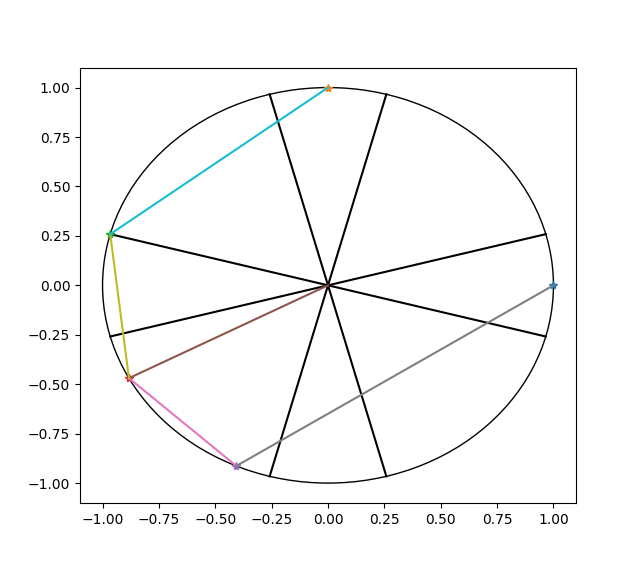
\includegraphics[scale=0.4]{5eme_cas1}
  \caption{Résolution 5e cas n1}
  \label{fig:5eme_cas1}
\end{figure}

Nous sommes ici encore en capacité d'utiliser \ref{worstchord}

\label{5cas13} Dans le cas où les deux sont entre A et C on a

\begin{figure}[h!]
  \centering
  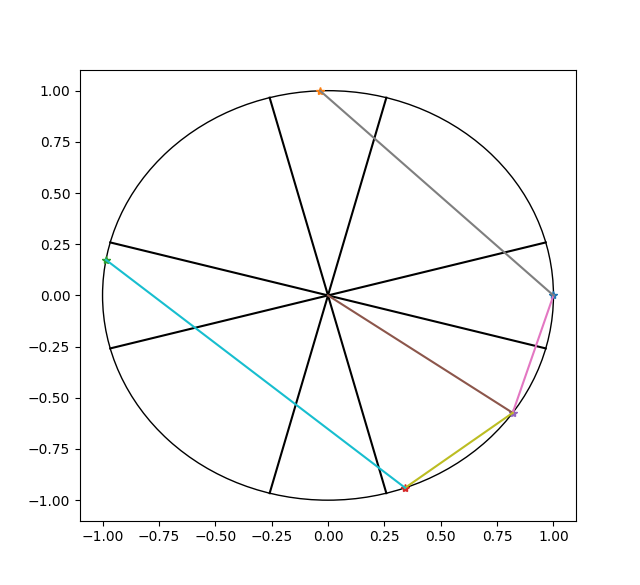
\includegraphics[scale=0.4]{5eme_cas1bis}
  \caption{Résolution 5e cas n1bis}
  \label{fig:5eme_cas1bis}
\end{figure}

grâce à l'écart d'angle entre les points, on a bien encore une fois les conditions d'applications de \ref{worstchord}

\end{itemize}

\item \label{5cas2} Si le point dans D appartient au demi-cercle du bas, on a 4 cas

\begin{itemize}

\item \label{5cas21} si point libre du haut entre A et B et point du bas entre A et C

\begin{figure}[h!]
  \centering
  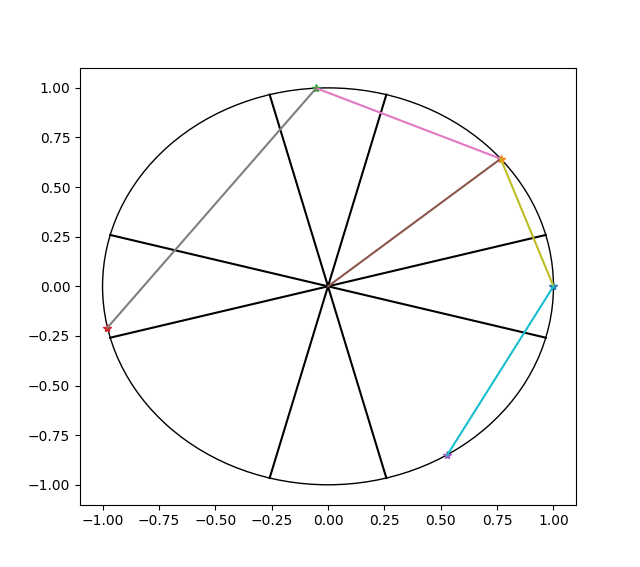
\includegraphics[scale=0.4]{5eme_cas2}
  \caption{Résolution 5e cas n2}
  \label{fig:5eme_cas2}
\end{figure}

en oubliant pas que le point de départ est forcément éloigné d'un angle $\alpha$ de $a$ on a bien le résultat par \ref{worstchord}

\item \label{5cas22} si point libre du haut entre A et B et point du bas entre C et D alors cela dépend de $b$. Si $b$ est sur le côté droit, on commence effectue cet arbre:

\begin{figure}[h!]
  \centering
  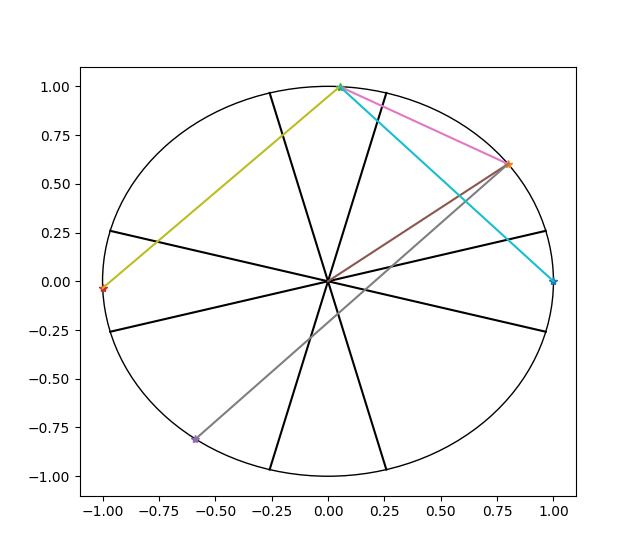
\includegraphics[scale=0.4]{5eme_cas3}
  \caption{Résolution 5e cas n3}
  \label{fig:5eme_cas3}
\end{figure}

on a alors

$\gamma(P) \leq \max\left(1+2\chord\left(\frac{\pi}{2} - \frac{\alpha}{4}\right), 1 + \chord\left(\frac{\pi}{2} - \alpha\right) + \chord\left(\frac{\pi}{2}\right)\right) \leq 1+2\chord\left(\frac{\pi}{2} - \frac{\alpha}{4}\right)$

si maintenant $b$ est sur le côté gauche, on peut commencer par $b$. On effectuant un arbre classique, le côté gauche a la bonne borne et le côté droit est facile

\item \label{5cas23} si point libre du haut entre B et D et point libre du bas entre C et D on a l'arbre suivant.

\begin{figure}[h!]
  \centering
  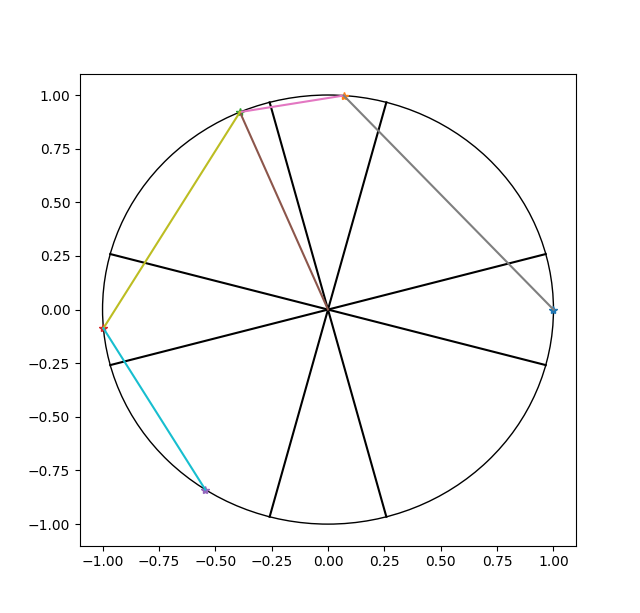
\includegraphics[scale=0.4]{5eme_cas4}
  \caption{Résolution 5e cas n4}
  \label{fig:5eme_cas4}
\end{figure}

\item \label{5cas24} si point libre du haut entre B et D et point libre du bas entre A et C cela dépend à nouveau de $b$. Si $b$ à droite on a (en allant vers le point le plus proche):

\begin{figure}[h!]
  \centering
  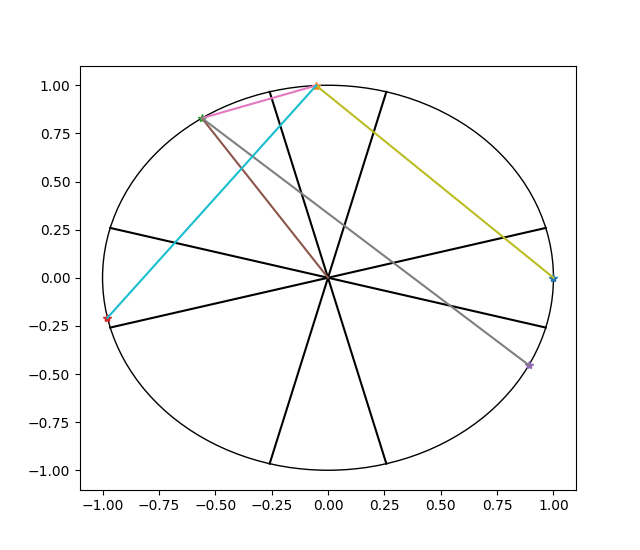
\includegraphics[scale=0.4]{5eme_cas5}
  \caption{Résolution 5e cas n5}
  \label{fig:5eme_cas5}
\end{figure}

en effet, on obtient alors en allant vers le plus proche que la longueur de la branche qui effectue le croisement est plus petite que $1+\chord\left(\frac{\frac{\pi}{2} + \frac{\alpha}{2}}{2}\right) + \chord\left(\frac{\pi}{4} + \frac{\alpha}{4}\right)$ or cette valeur est inférieure à $\max\left(3 + \chord\left(\alpha\right), 1 + 2\chord\left(\frac{\pi}{2} - \frac{\alpha}{4}\right)\right)$ on a alors le résultat souhaité.

cependant si $b$ est à gauche on peut alors commencer par $b$ pour finir le problème comme la dernière fois.

\end{itemize}
\end{itemize}

\subsection{convexe de taille 4 ou 3}\label{conv3}

Désormais, il faut terminer avec les cas où l'enveloppe convexe est de taille 3 ou 4. Heureusement, ces cas sont plus simples.
Si l'enveloppe convexe est de taille 3, on va vers le point le plus proche du centre qui soit à l'intérieur de l'enveloppe convexe, ensuite un des deux robots ira chercher le deuxième point à l'intérieur tandis que le deuxième ira réveiller le point le plus proche du triangle avant d'aller sur les deux autres.

\begin{figure}[h!]
  \centering
  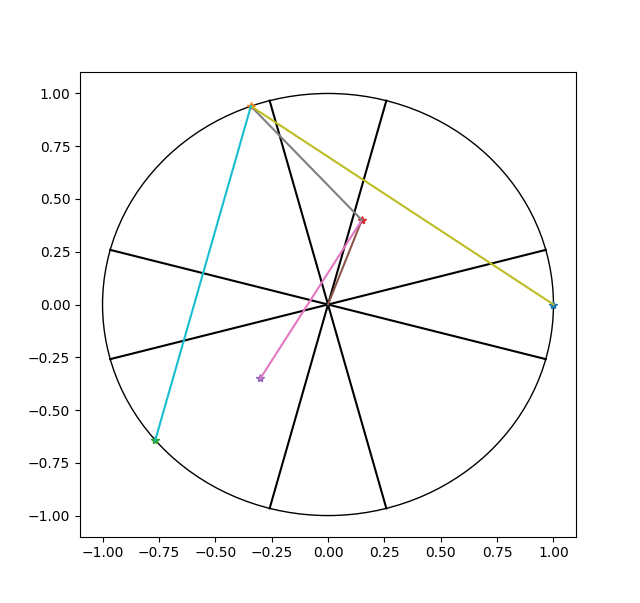
\includegraphics[scale=0.4]{n3}
  \caption{Résolution Pour une enveloppe convexe de taille 3}
  \label{fig:n3}
\end{figure}

En effet, le pire cas est si le point que l'on rejoint en premier est projeté sur l'enveloppe convexe orthogonalement ce qui nous donne $\exists \theta, \gamma(P) \leq \cos(\theta) + \sin(\theta) + 2 \leq \sqrt{2} + 2 \leq \max(3 + \chord(\alpha), 1 + 2\chord(\frac{\pi}{2} - \frac{\alpha}{4}))$

Note: En réalité, cela fonctionne quelque soit l'emplacement du deuxième point à l'intérieur, et donc également si il n'est pas dans l'enveloppe connexe, et il est donc possible de traiter par exactement la même méthode le cas où l'enveloppe convexe est de taille 4.

\subsection{conclusion of the proof}

Cela conclut la preuve, trouvant ainsi une borne pour $\alpha_5$ montrant également que $\alpha_5 < \alpha_4$. On remarquera que plus on fait de disjonctions de cas, plus il est possible d'affiner le choix de l'arbre selon les situations, permettant ainsi d'obtenir une meilleure borne.